% Copyright 2004 by Till Tantau <tantau@users.sourceforge.net>.
%
% In principle, this file can be redistributed and/or modified under
% the terms of the GNU Public License, version 2.
%
% However, this file is supposed to be a template to be modified
% for your own needs. For this reason, if you use this file as a
% template and not specifically distribute it as part of a another
% package/program, I grant the extra permission to freely copy and
% modify this file as you see fit and even to delete this copyright
% notice. 

\documentclass{beamer}
\usepackage{subfig}

% There are many different themes available for Beamer. A comprehensive
% list with examples is given here:
% http://deic.uab.es/~iblanes/beamer_gallery/index_by_theme.html
% You can uncomment the themes below if you would like to use a different
% one:
%\usetheme{AnnArbor}
%\usetheme{Antibes}
%\usetheme{Bergen}
%\usetheme{Berkeley}
%\usetheme{Berlin}
%\usetheme{Boadilla}
%\usetheme{boxes}
%\usetheme{CambridgeUS}
%\usetheme{Copenhagen}
%\usetheme{Darmstadt}
%\usetheme{default}
%\usetheme{Frankfurt}
%\usetheme{Goettingen}
%\usetheme{Hannover}
%\usetheme{Ilmenau}
%\usetheme{JuanLesPins}
%\usetheme{Luebeck}
\usetheme{Madrid}
%\usetheme{Malmoe}
%\usetheme{Marburg}
%\usetheme{Montpellier}
%\usetheme{PaloAlto}
%\usetheme{Pittsburgh}
%\usetheme{Rochester}
%\usetheme{Singapore}
%\usetheme{Szeged}
%\usetheme{Warsaw}

\title{CopyNET - Incorporating Copying Mechanism in Seq2Seq Learning}

% A subtitle is optional and this may be deleted
\subtitle{Jiatao Gu, Zhengdong Lu, Hang Li, Victor O.K. Li 2016 }

\author{Louis (Yiqing) Luo}
% - Give the names in the same order as the appear in the paper.
% - Use the \inst{?} command only if the authors have different
%   affiliation.

\institute[University of Toronto] % (optional, but mostly needed)


\date{Aug 3rd, 2018}
% - Either use conference name or its abbreviation.
% - Not really informative to the audience, more for people (including
%   yourself) who are reading the slides online


% Delete this, if you do not want the table of contents to pop up at
% the beginning of each subsection:
\AtBeginSubsection[]
{
  \begin{frame}<beamer>{Outline}
    \tableofcontents[currentsection,currentsubsection]
  \end{frame}
}

% Let's get started
\begin{document}

\begin{frame}
  \titlepage
\end{frame}



% Section and subsections will appear in the presentation overview
% and table of contents.

\section{Motivation}
\begin{frame}{Motivation}
    \begin{itemize}
        \item Problem: Copying in Seq2Seq
        
        \begin{itemize}
            \item  certain segments in the input sequence are selectively replicated in the output sequence
            \item eg. humans tend to repeat ntity names or even long phrases in conversation
        \end{itemize}
        
        \begin{figure}
            \centering 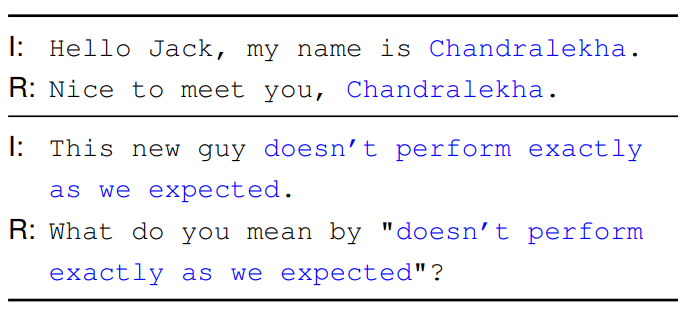
\includegraphics{eg.PNG}
        \end{figure}
    \end{itemize}
    
\end{frame}

\begin{frame}{Motivation}
\begin{itemize}
   \item Problem: Copying in Seq2Seq
        
        \begin{itemize}
            \item  certain segments in the input sequence are selectively replicated in the output sequence
            \item eg. humans tend to repeat entity names or even long phrases in conversation
        \end{itemize}
\end{itemize} 
Proposed Solution:     
\begin{center}
    CopyNET = RNN Encoder $\&$ Decoder + Copying Mechanism
\end{center}
    
\end{frame}

%\subsection{Matrix Multiplication on Input Vectors}
\begin{frame}{RNNSearch: RNN Encoder and Decoder}
    \begin{itemize}
        \item typically used in Seq2Seq learning
    \end{itemize}
    \begin{figure}
        \centering
        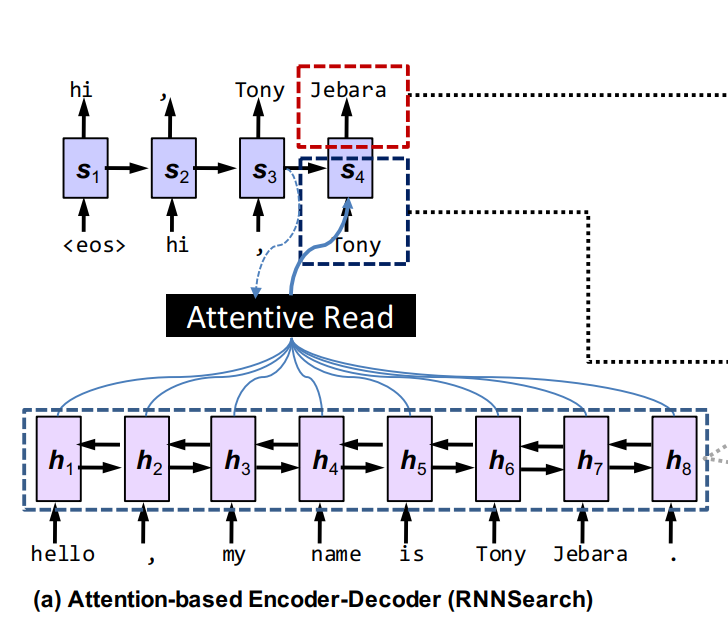
\includegraphics[width=0.6\textwidth]{rnnsearc.PNG}
    \end{figure}
        
\end{frame}

\begin{frame}{CopyNET}
    Encoder same.
    Decoder Differences:
    \begin{enumerate}
        \item \textbf{Prediction:} COPYNET predicts words based on a mixed probabilistic model of two modes 
        \item \textbf{State Update:} uses not only its word-embedding but also its corresponding location-specific hidden state in M
        %\item \textbf{Reading M:} hybrid of content-based addressing and location-based addressing
    \end{enumerate}
    \pause
    \begin{figure}
        \centering
        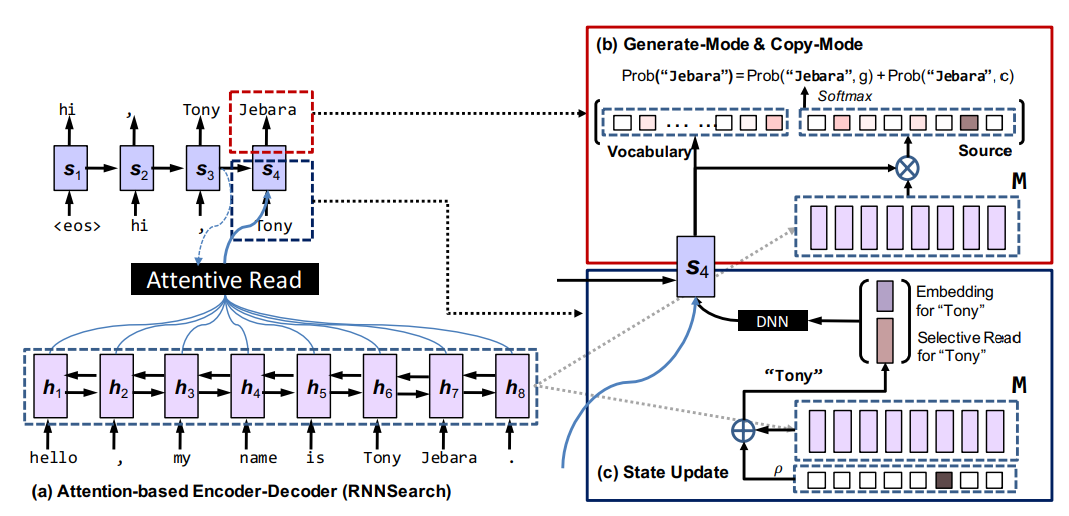
\includegraphics[scale = 0.6]{copynet.PNG}
    \end{figure}
\end{frame}

\begin{frame}{Model}
\begin{figure}
        \centering
        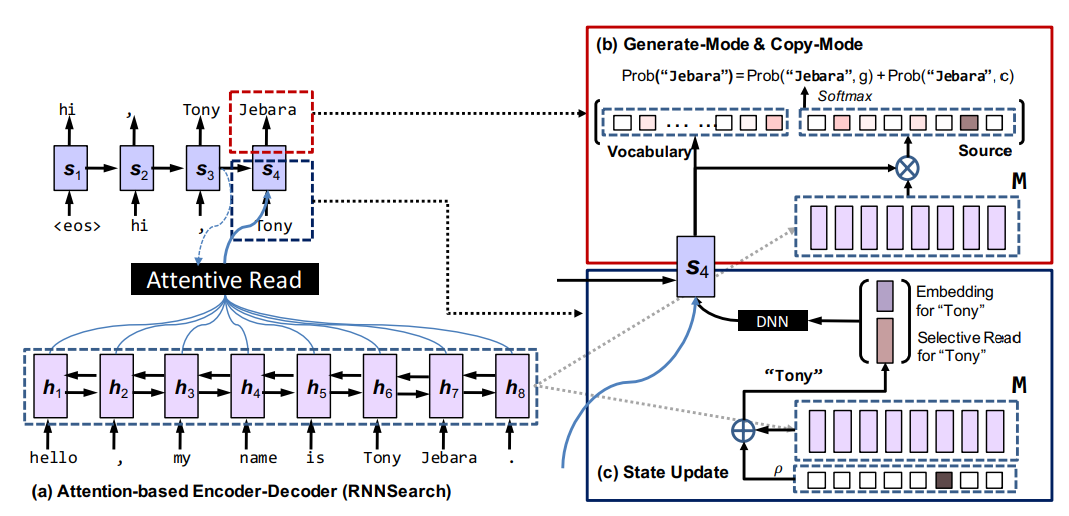
\includegraphics[width = \textwidth]{copynet.PNG}
\end{figure}
\end{frame}

%\subsection{Scalar Weighting - Dynamic Routing}
\begin{frame}{Decoder: 1. Prediction}
    \begin{itemize}
        \item For vocabulary \textit{V} and unique words in source sequence \textit{X}
        \item Instance-specific Vocabulary for source X is $\textit{V} \cup UNK \cup \textit{X}$
    \end{itemize}
    Given the decoder RNN state $\textbf{s}_t$ at time t together with \textbf{M}, the probability of generating any target word $y_t$, is given by the “mixture” of probabilities as follows:
    \begin{figure}
        \centering
        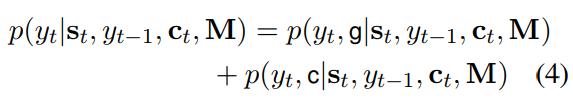
\includegraphics{pred_eq.PNG}
    \end{figure}
\end{frame}

\begin{frame}{Equations Unrolled:}
    \begin{figure}
        \centering
        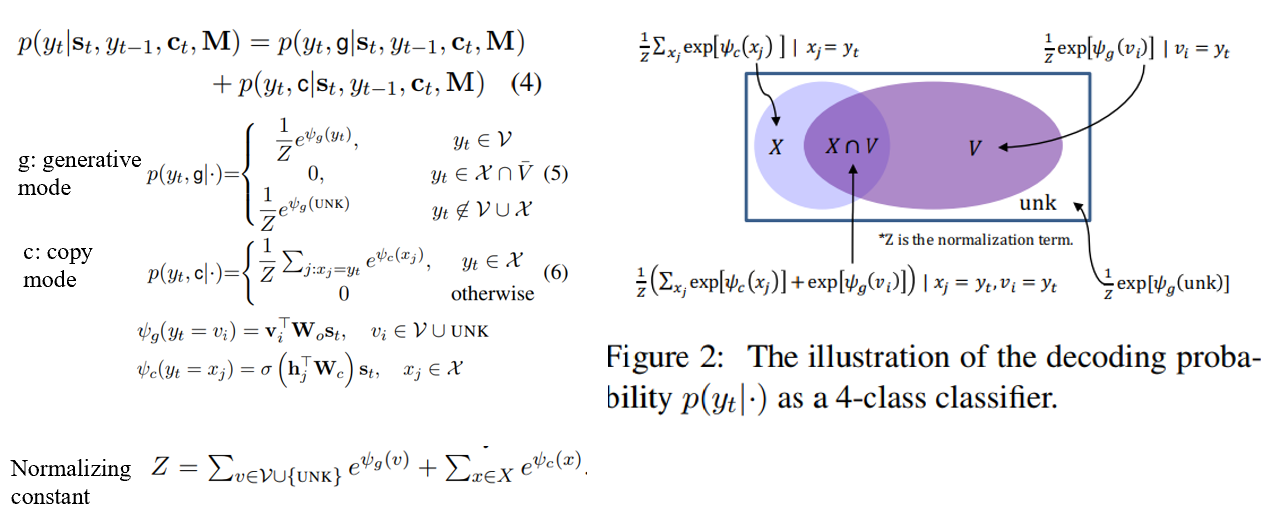
\includegraphics[width = 1.05\linewidth]{pred_eq_all.PNG}
    \end{figure}
       
\end{frame}

%\subsection{Squash for Non-Linearity}
\begin{frame}{Experiments - Language Modeling}
\begin{figure}
    \centering
    \includegraphics{table5.JPG}
\end{figure}
\end{frame}

%\subsection{Experiments - Size of Training Data (German and English)}
\begin{frame}{Decoder: 2. State Update}
\begin{itemize}
    \item normally $\textbf{s}_t$ is updated by {$\textbf{s}_{t-1}, y_{t-1}, and \textbf{c}_t$}
    \item with CopyNET: the $y_{t-1}$ in $y_{t-1} \rightarrow \textbf{s}_{t}$ is replaced with: 
\end{itemize}
    \begin{figure}
    \centering
    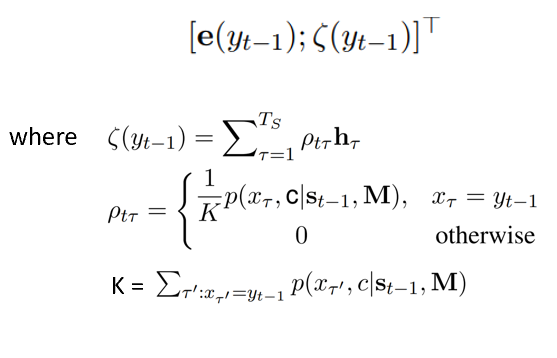
\includegraphics[scale = 0.7]{state_update_full.PNG}
\end{figure}
where $\textbf{e}(y_t−1)$ is the word embedding associated with $y_t−1$, while $\zeta(y_t−1)$ is the weighted sum of hidden states in \textbf{M} corresponding to $y_t$
\end{frame}

%\section{Size of n-Gram}
%\subsection{Capsule Network Encoder Architecture}
\begin{frame}{Loss function and Updating}
    \begin{figure}
        \centering
        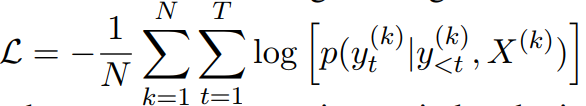
\includegraphics[scale = 0.85]{loss.PNG}
    \end{figure}
    where source sequence = $X^{(N)}$ and target sequence = $Y^{(N)}$
    \begin{itemize}
        \item  The network can learn to coordinate
the two modes from data
        \begin{itemize}
            \item if a target word in the source sequence, the copy-mode will contribute
        to the mixture model, and the gradient will
        more or less encourage the copy-mode; otherwise,
        the copy-mode is discouraged due to the competition
        from the shared normalization term Z
        \end{itemize}
    \end{itemize}
\end{frame}

%\subsection{Loss Function for Encoder}
\begin{frame}{Experiment}
    \begin{enumerate}
        \item A synthetic dataset on with simple patterns;
        \item A real-world task on text summarization;
        \item A dataset for simple single-turn dialogues.
    \end{enumerate}
\end{frame}

\begin{frame}{Experiments - Synthetic Dataset}
Each rule can further produce a number
of instances by replacing the variables with
randomly generated subsequences (1 to 15 symbols)
from the same vocabulary
\begin{figure}
    \centering
    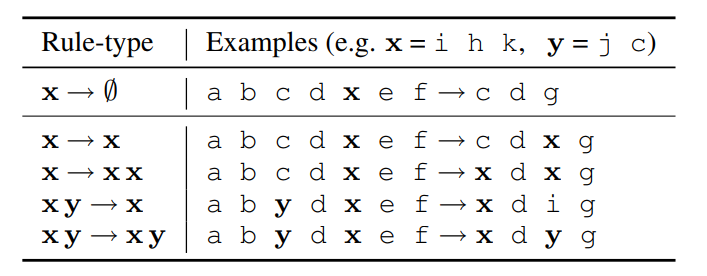
\includegraphics[scale=0.9]{syn_rule.PNG}
\end{figure}
\end{frame}

\begin{frame}{Experiments - Synthetic Dataset}
\begin{figure}
    \centering
    \includegraphics[scale=0.9]{table8.JPG}
\end{figure}
\begin{itemize}
    \item Encoder-Decoder (no Attention) $\rightarrow$  difficulty of representing a long sequence with very high fidelity
    \item RNNSearch (with Attention) $\rightarrow$ attention alone seems inadequate for handling the case where strict replication is needed
\end{itemize}
\end{frame}

%\subsection{Pretrained models}
\begin{frame}{Experiments - Text Summarization}
    Automatic text summarization aims to find a condensed representation which can capture the core meaning of the original document
    \begin{itemize}
        \item Dataset:  LCSTS dataset (Hu et al., 2015), a large scale dataset for short text summarization in form of (short news, summary).
        \item model tried on character (+C) and word (+W)
        \item ROUGE-N: Overlap of N-grams between the system and reference summaries.
        \item ROUGE - LCN: measures longest matching sequence of words using longest common subsequence.
    \end{itemize}
    \begin{figure}
        \centering
        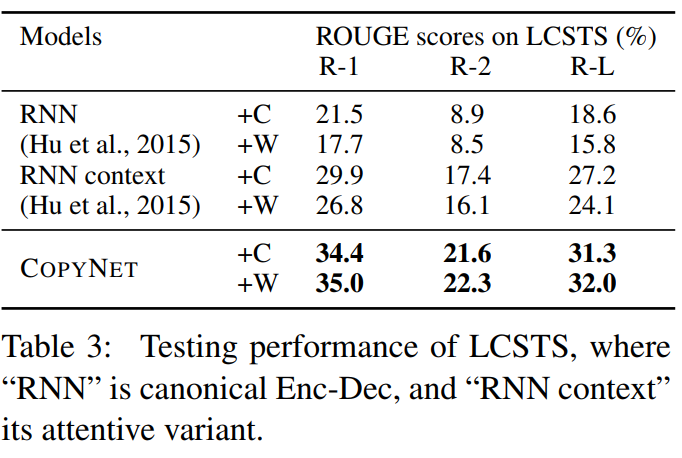
\includegraphics[scale=0.7]{sum_result.PNG}
    \end{figure}
\end{frame}

\begin{frame}{Experiments - Text Summarization}
\begin{figure}
    \centering
    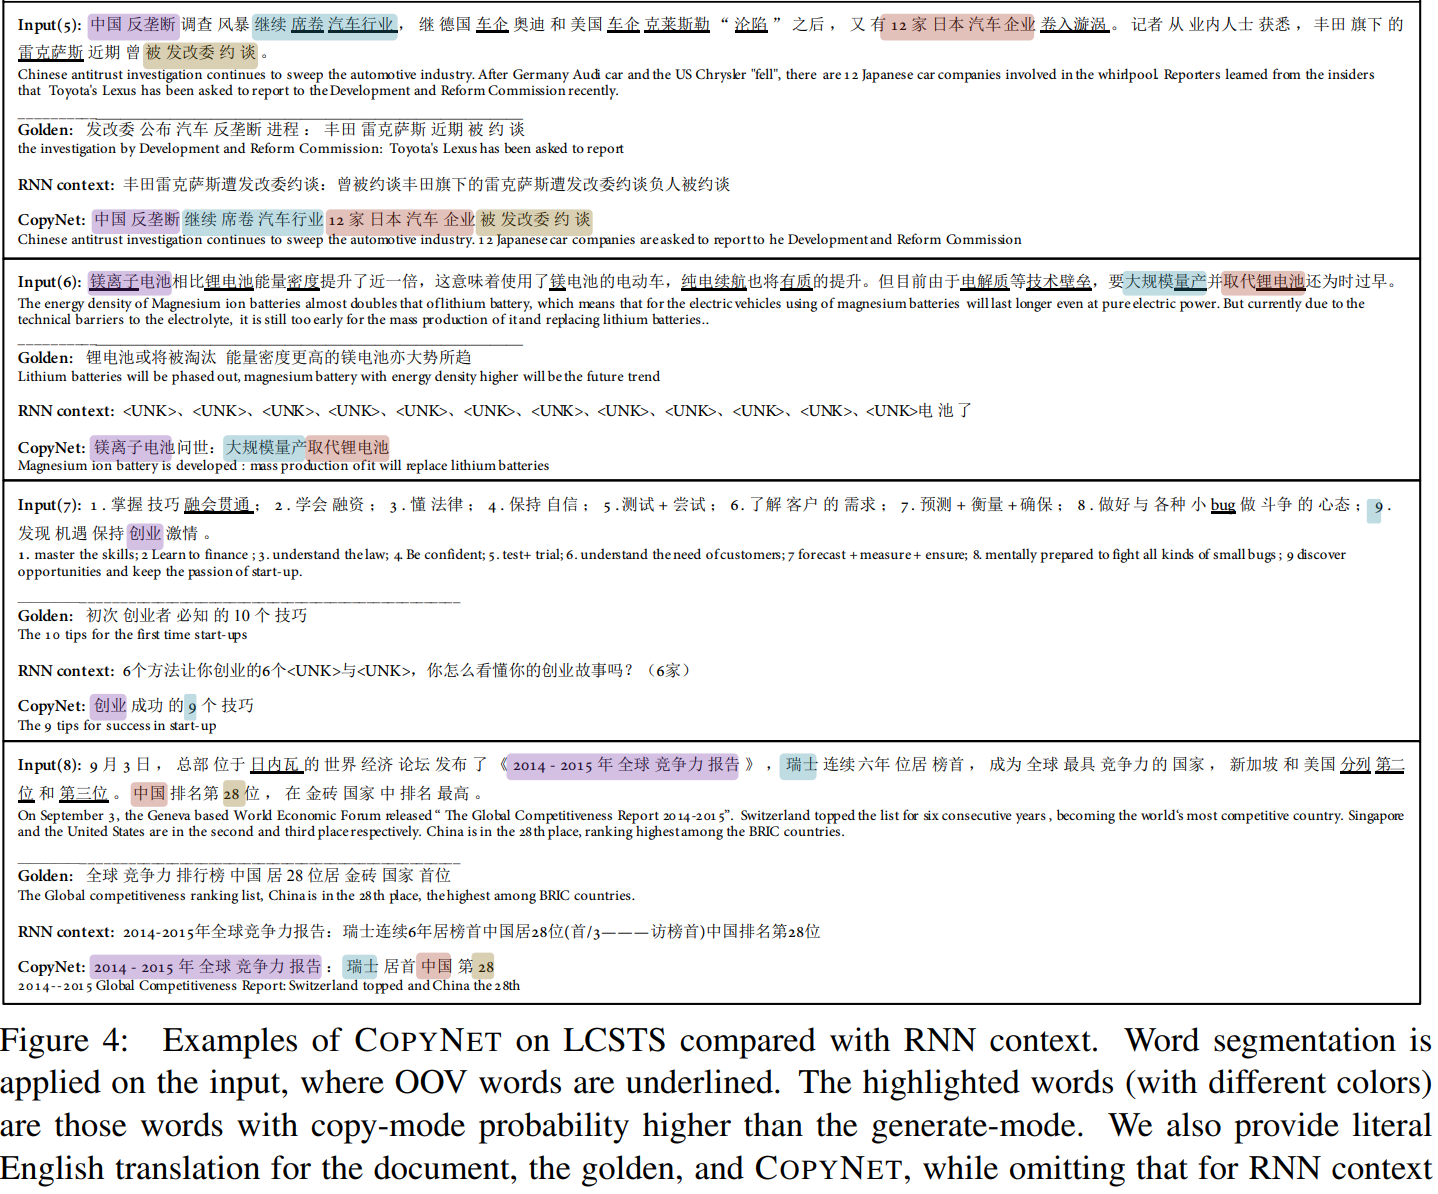
\includegraphics[height=0.9\textheight]{sum_ex2.PNG}
\end{figure}
\end{frame}

\begin{frame}{Experiments - Text Summarization}
    \begin{enumerate}
    \item most words are from copy-mode,
but the summary is usually still fluent; 
\item COPYNET
tends to cover consecutive words in the original
document, but it often puts together segments
far away from each other, indicating a sophisticated
coordination of content-based addressing
and location-based addressing; 
\item COPYNET
handles OOV words really well: it can generate
acceptable summary for document with many
OOVs, and even the summary itself often contains
many OOV words
\end{enumerate}
\end{frame}

\begin{frame}{Experiments - Single-turn Dialogue}
    \begin{itemize}
        \item {Dataset built via a simple dialogue dataset
based on the following three instructions}
        \begin{enumerate}
            \item {Dialogue instances are collected from Baidu
            Tieba3 with some coverage of conversations
            of real life e.g., greeting and sports, etc.}
            \item {patterns with slots like \begin{center}
                hi, my name is x → hi, x
            \end{center}
            are mined from the set, with possibly multiple
            responding patterns to one input.}
            \item {Similar with the synthetic dataset, we enlarge
            the dataset by filling the slots with suitable
            subsequence (e.g. name entities, dates, etc.)}
        \begin{itemize}
            \item Created 2 datasets: DS-I and DS-II
            \item the filled substrings for training and
        testing in DS-II have no overlaps, while in DS-I
        they are sampled from the same pool
        \end{itemize}
        \end{enumerate}
    \end{itemize}
\end{frame}

\begin{frame}{Experiments - Single-turn Dialogue}
    \begin{figure}
        \centering
        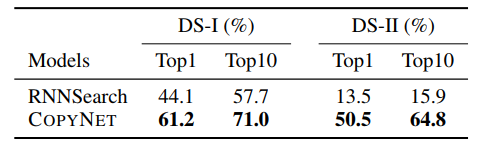
\includegraphics{dia_results.PNG}
    \end{figure}
    \begin{itemize}
        \item Both models estimate respectively
the chance of the top-1 or one of top-10 (from
beam search) matching the golden.
    \end{itemize}
\end{frame}

\begin{frame}{Experiments - Single-turn Dialogue}
    \begin{figure}
        \centering
        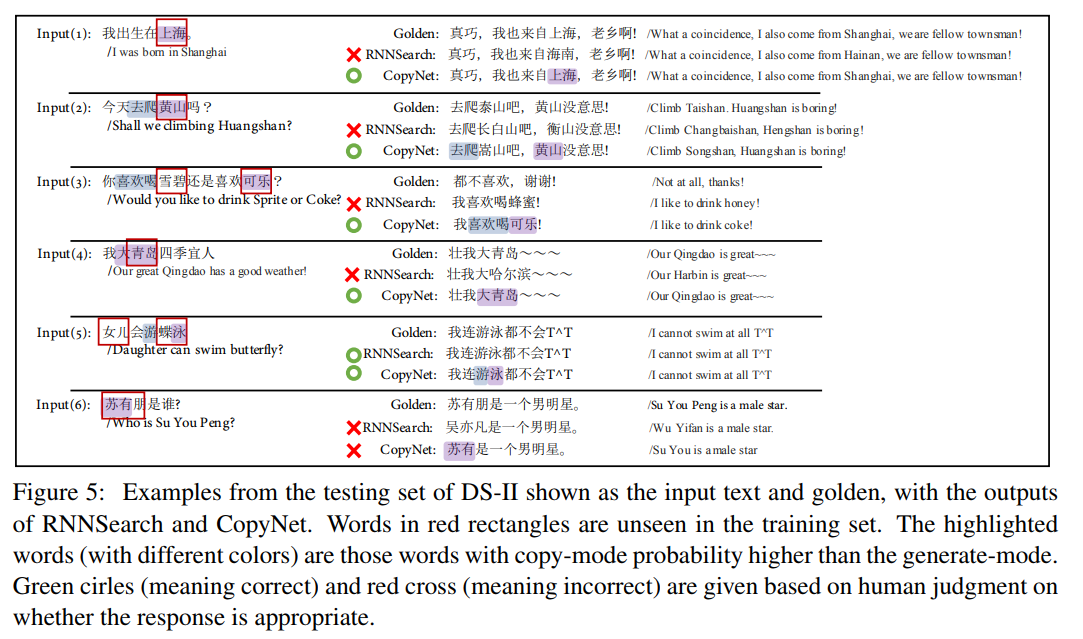
\includegraphics[height=0.8\textheight]{dia_ex.PNG}
    \end{figure}
\end{frame}


\end{document}




